\documentclass[11pt,a4paper]{article}
\usepackage[T1]{fontenc}
\usepackage[utf8]{inputenc}
\usepackage[brazil]{babel}
\usepackage{lmodern}
\usepackage[margin=2.2cm]{geometry}
\usepackage{graphicx}
\usepackage{booktabs}
\usepackage{float}
\usepackage{caption}
\usepackage{xcolor}
\usepackage{listings}
\usepackage{array}
\usepackage{upquote}
\usepackage[hidelinks]{hyperref}

\graphicspath{{../}}

\lstset{
  basicstyle=\ttfamily\footnotesize,
  backgroundcolor=\color{gray!8},
  frame=single, rulecolor=\color{gray!40},
  breaklines=true, columns=fullflexible, showstringspaces=false, upquote=true,
  keywordstyle=\color{blue!60!black}\bfseries,
  commentstyle=\color{gray}\itshape,
  stringstyle=\color{red!50!black},
  literate={ã}{{\~a}}1 {ç}{{\c{c}}}1 {õ}{{\~o}}1 {é}{{\'e}}1 {á}{{\'a}}1 {í}{{\'i}}1 {ú}{{\'u}}1 {ê}{{\^e}}1
}

\newcommand{\col}[1]{\texttt{#1}}

\title{PCS5916 - Computação de Alto Desempenho e Aplicações\\[4pt]
\large Exercícios Aula 05 - Apache Spark\\
Food Establishment Inspection Data (King County)}
\author{Andre Moreno Goveia - 13682785}

\begin{document}
\maketitle

\section*{Etapas realizadas}

\begin{enumerate}
  \item \textbf{Cluster.} Foi utilizado o cluster Amazon EMR \textit{ClusterAndreLab1} (EMR 7.14.0, Spark 3.5.8, JupyterHub 1.5.0), com 1 nó primário e 2 nós \textit{core} (Figura~\ref{fig:emr}).
  \item \textbf{Dados.} A versão atualizada do conjunto \textit{Food Establishment Inspection Data} foi baixada do portal de dados de King County (arquivo \col{Food\_Establishment\_Inspection\_Data\_20261022.csv}, 31,9~MB) e enviada para \col{s3://bucket-andre-lab1/}.
  \item \textbf{Notebook.} O processamento foi feito no notebook PySpark (kernel \textit{PySpark}, via Livy) \col{restaurants\_spark.ipynb}: leitura do CSV no S3, padronização dos nomes de colunas, conversão de tipos, \textit{cache} do DataFrame, registro da visão temporária \col{restaurant\_violations} e consultas em Spark SQL.
  \item \textbf{Saída.} Os resultados das questões 2, 3 e 4 foram gravados em CSV em \col{s3://bucket-andre-lab1/output/} (Figura~\ref{fig:s3}).
  \item \textbf{Spark UI.} A execução foi examinada pelo \textit{Spark History Server} (\textit{Persistent application UI} do console do EMR), já que o endereço interno do driver (\col{ip-172-31-41-100.ec2.internal}) não é acessível fora da VPC.
\end{enumerate}

\begin{figure}[H]
  \centering
  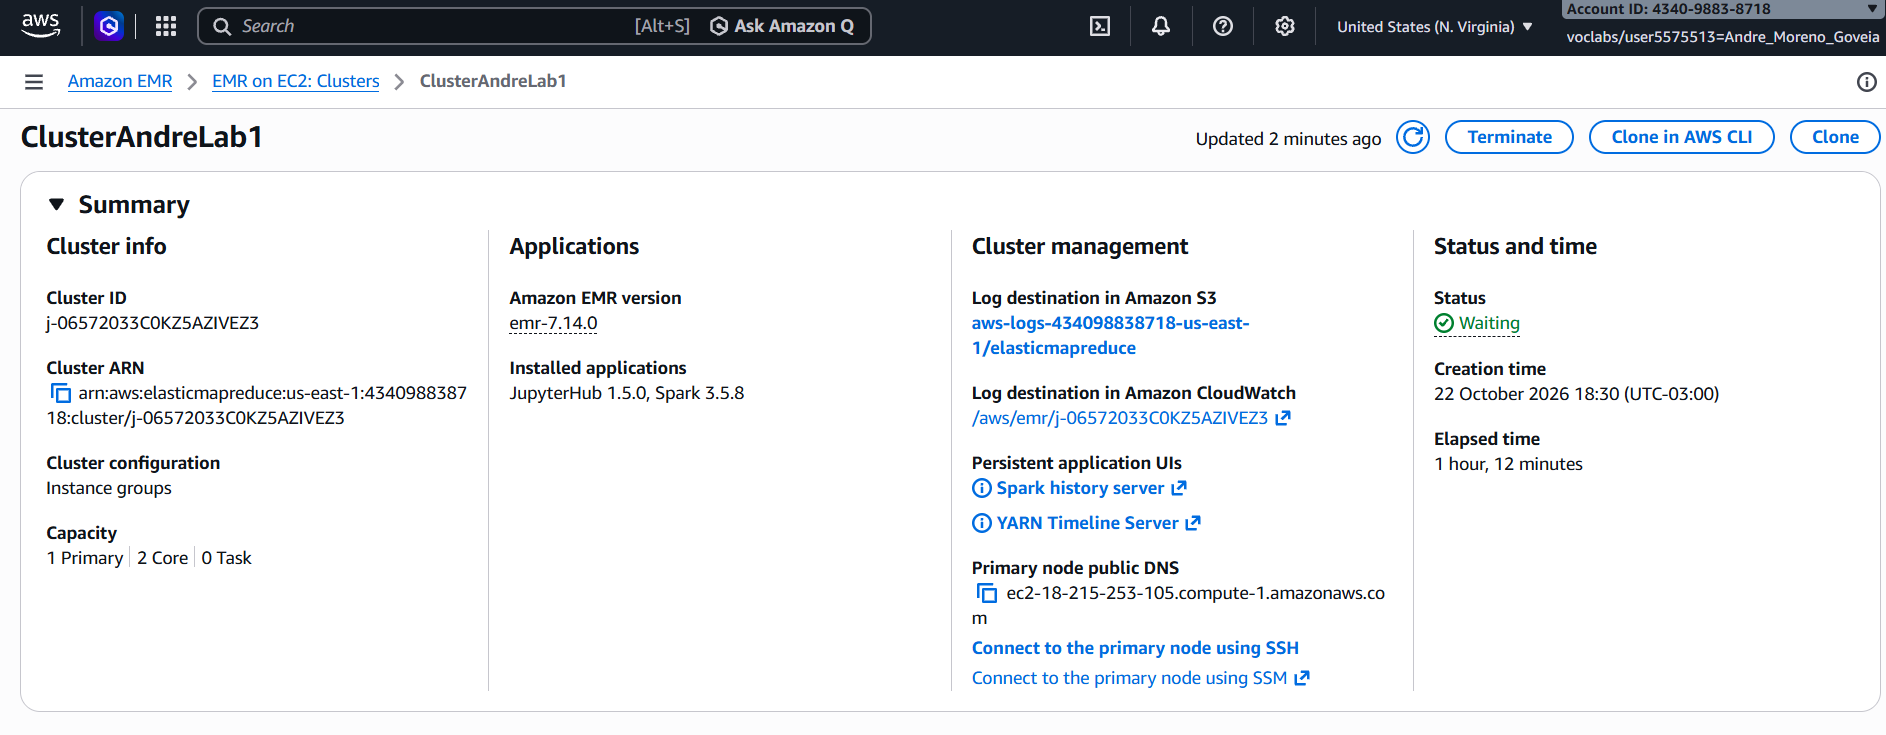
\includegraphics[width=\linewidth]{emr_summary.png}
  \caption{Resumo do cluster EMR utilizado.}
  \label{fig:emr}
\end{figure}

\begin{figure}[H]
  \centering
  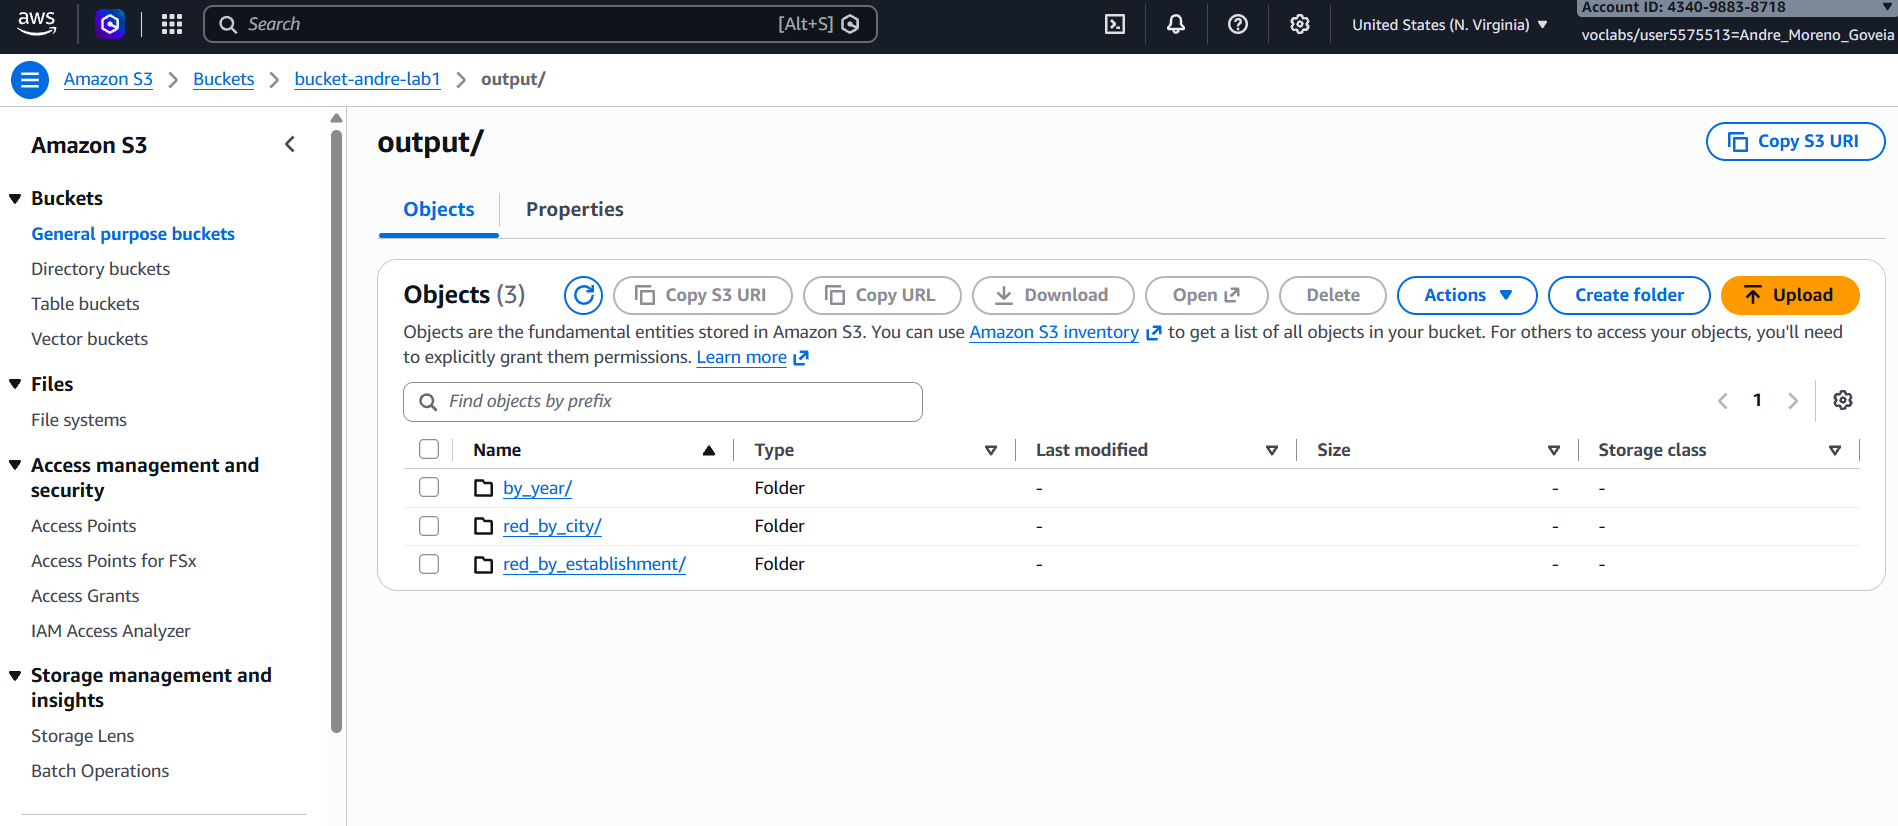
\includegraphics[width=0.85\linewidth]{output_s3.png}
  \caption{Resultados gravados no Amazon S3 (\col{output/}).}
  \label{fig:s3}
\end{figure}

% ---------------------------------------------------------------
\section{Estrutura e qualidade dos dados}

O conjunto atualizado possui \textbf{110.068 registros} e \textbf{20 colunas}, com inspeções de \textbf{04/01/2021 a 21/10/2026}. Cada linha corresponde a \emph{uma infração} registrada em uma inspeção; inspeções sem infração aparecem em uma única linha com \col{violation\_type} nulo. Assim, a mesma inspeção (\col{inspection\_serial\_num}) pode ocupar várias linhas: há 74.129 inspeções únicas e 12.301 estabelecimentos (\col{business\_id}).

\begin{table}[H]
\centering
\small
\caption{Colunas, tipos (após conversão) e valores ausentes.}
\begin{tabular}{llrr}
\toprule
Coluna original & Coluna / tipo no Spark & Ausentes & \% \\
\midrule
Name & \col{name} / string & 0 & 0,0 \\
Program Identifier & \col{program\_identifier} / string & 90.323 & 82,1 \\
Inspection Date & \col{inspection\_date} / date & 0 & 0,0 \\
Classification & \col{classification} / string & 0 & 0,0 \\
Address & \col{address} / string & 0 & 0,0 \\
City & \col{city} / string & 9 & 0,0 \\
Zip Code & \col{zip\_code} / string & 0 & 0,0 \\
Inspection Type & \col{inspection\_type} / string & 0 & 0,0 \\
Inspection Score & \col{inspection\_score} / integer & 0 & 0,0 \\
Inspection Result & \col{inspection\_result} / string & 0 & 0,0 \\
Inspection Closed Business & \col{inspection\_closed\_business} / boolean & 0 & 0,0 \\
Seating Range & \col{seating\_range} / string & 23.800 & 21,6 \\
Risk Category & \col{risk\_category} / integer & 676 & 0,6 \\
Violation Type & \col{violation\_type} / string & 41.011 & 37,3 \\
Violation Description & \col{violation\_description} / string & 41.011 & 37,3 \\
Violation Points & \col{violation\_points} / integer & 0 & 0,0 \\
Grade & \col{grade} / string & 0 & 0,0 \\
Parcel Number & \col{parcel\_number} / string & 465 & 0,4 \\
Business\_ID & \col{business\_id} / string & 0 & 0,0 \\
Inspection\_Serial\_Num & \col{inspection\_serial\_num} / string & 0 & 0,0 \\
\bottomrule
\end{tabular}
\end{table}

Os 41.011 nulos em \col{violation\_type} e \col{violation\_description} são as inspeções sem infração. A distribuição de \col{violation\_type} é RED = 34.244, BLUE = 34.813 e nulo = 41.011; a de \col{inspection\_result} é Satisfactory = 53.790, Unsatisfactory = 53.499 e Complete = 2.779. A coluna \col{city} tem 9 nulos e grafias inconsistentes (por exemplo, \textit{Auburn}/\textit{AUBURN} e o erro de digitação \textit{BELLEUE}).

\subsection*{Alterações no código em relação ao laboratório}

\begin{table}[H]
\centering
\small
\begin{tabular}{>{\raggedright\arraybackslash}p{4.3cm}>{\raggedright\arraybackslash}p{5.2cm}>{\raggedright\arraybackslash}p{5.8cm}}
\toprule
Laboratório & Dataset atualizado & Ajuste no código \\
\midrule
\addlinespace
5 colunas em \textit{snake\_case} (\col{name}, \col{violation\_type}, \ldots) & 20 colunas com espaços e maiúsculas (\col{Violation Type}, \col{Inspection Date}, \ldots) & Renomear todas as colunas para \textit{snake\_case} com \col{toDF} \\
Sem data, cidade ou identificador de inspeção & \col{Inspection Date}, \col{City}, \col{Business\_ID}, \col{Inspection\_Serial\_Num} & Possibilitam as análises por cidade, por ano e por inspeção única \\
\col{inferSchema} suficiente & Data em \col{MM/dd/yyyy}; códigos com zeros à esquerda (\col{Zip Code}, \col{Parcel Number}) & Ler tudo como string e converter explicitamente (\col{to\_date}, \col{cast("int")}) \\
\col{inspection\_closed\_}\-\col{business} = TRUE/FALSE & Yes/No & Converter para booleano \\
Não havia cidade & Mesma cidade com grafias diferentes & \col{upper(trim(city))}; o mesmo em \col{violation\_type} \\
Agrupamento por \col{name} & \col{Business\_ID} identifica cada estabelecimento & Agrupar por \col{business\_id} na questão 2 \\
\bottomrule
\end{tabular}
\end{table}

\begin{lstlisting}[language=Python]
raw_df = spark.read.option("header", "true").csv(data_source)
raw_df = raw_df.toDF(*[c.strip().lower().replace(" ", "_") for c in raw_df.columns])

restaurants_df = (raw_df
    .withColumn("inspection_date", F.to_date("inspection_date", "MM/dd/yyyy"))
    .withColumn("inspection_score", F.col("inspection_score").cast("int"))
    .withColumn("violation_points", F.col("violation_points").cast("int"))
    .withColumn("risk_category", F.col("risk_category").cast("int"))
    .withColumn("inspection_closed_business", F.col("inspection_closed_business") == "Yes")
    .withColumn("city", F.upper(F.trim("city")))
    .withColumn("violation_type", F.upper(F.trim("violation_type")))
    .cache())
restaurants_df.createOrReplaceTempView("restaurant_violations")
\end{lstlisting}

% ---------------------------------------------------------------
\section{Infrações RED por estabelecimento}

\begin{lstlisting}[language=SQL]
SELECT business_id, first(name) AS name, first(address) AS address, first(city) AS city,
       COUNT(*) AS total_red_violations,
       COUNT(DISTINCT inspection_serial_num) AS inspections_with_red
FROM restaurant_violations
WHERE violation_type = 'RED'
GROUP BY business_id
ORDER BY total_red_violations DESC
LIMIT 10
\end{lstlisting}

\begin{table}[H]
\centering
\small
\caption{Top 10 estabelecimentos (por \col{business\_id}) com mais registros de infrações RED.}
\begin{tabular}{rllrrr}
\toprule
\# & Estabelecimento & Cidade & Registros RED & Inspeções c/ RED & RED/inspeção \\
\midrule
1 & Bombay Grill & Seattle & 53 & 12 & 4,4 \\
2 & Red Onion Tavern & Seattle & 50 & 12 & 4,2 \\
3 & Ruchi Indian Restaurant & Bellevue & 46 & 15 & 3,1 \\
4 & Patio Fine Thai Cuisine & Seattle & 45 & 16 & 2,8 \\
5 & Tian Fu & Seattle & 42 & 10 & 4,2 \\
6 & Tasty Szechuan & Bellevue & 42 & 12 & 3,5 \\
7 & Tiger Bites & Bellevue & 42 & 11 & 3,8 \\
8 & Mirch Masala Town & Kent & 39 & 8 & 4,9 \\
9 & Wicked Chopstix & Seattle & 38 & 10 & 3,8 \\
10 & 7-Eleven \#14396E (Sodhi Holdings) & Seattle & 37 & 14 & 2,6 \\
\bottomrule
\end{tabular}
\end{table}

Para comparação, a consulta do laboratório (agrupando apenas por \col{name}) produz outro ranking:

\begin{table}[H]
\centering
\small
\caption{Top 10 agrupando por nome (abordagem do laboratório).}
\begin{tabular}{rlr@{\hspace{1.5cm}}rlr}
\toprule
\# & Nome & RED & \# & Nome & RED \\
\midrule
1 & T-Mobile Park & 159 & 6 & Asian Pacific Market and Deli & 54 \\
2 & Subway & 154 & 7 & Bombay Grill & 53 \\
3 & Levy Restaurants @ Lumen Field & 130 & 8 & Red Onion Tavern & 50 \\
4 & Arena at Seattle Center & 63 & 9 & Taco del Mar & 50 \\
5 & PCC Community Markets & 59 & 10 & Just Poke & 49 \\
\bottomrule
\end{tabular}
\end{table}

\paragraph{Interpretação.} Agrupar por nome mistura volume com desempenho: T-Mobile Park, Lumen Field e Arena at Seattle Center são estádios com dezenas de pontos de venda inspecionados separadamente sob o mesmo nome, e Subway, PCC e Taco del Mar são redes com várias unidades. Esse era o mesmo efeito presente no resultado do laboratório (Subway, T-Mobile Park, Whole Foods no topo). Ao agrupar por \col{business\_id}, o ranking passa a mostrar estabelecimentos individuais, quase todos restaurantes independentes de Seattle, Bellevue e Kent, com predominância de cozinhas indiana, tailandesa e chinesa (preparo com muitos itens e controle de temperatura de alimentos quentes/frios, fontes comuns de infrações RED). O número de inspeções com RED (8 a 16 em cerca de cinco anos) e a média de 2,6 a 4,9 infrações RED por inspeção indicam \textbf{reincidência}: não são eventos isolados, e sim problemas que se repetem a cada visita. Como os valores são absolutos, estabelecimentos inspecionados com mais frequência tendem a acumular mais registros.

% ---------------------------------------------------------------
\section{Infrações RED por cidade}

\begin{lstlisting}[language=SQL]
SELECT city, COUNT(*) AS total_red_violations,
       ROUND(100 * COUNT(*) / SUM(COUNT(*)) OVER (), 2) AS pct_total
FROM restaurant_violations
WHERE violation_type = 'RED' AND city IS NOT NULL
GROUP BY city
ORDER BY total_red_violations DESC
LIMIT 10
\end{lstlisting}

\begin{table}[H]
\centering
\small
\caption{Top 10 cidades com mais registros de infrações RED.}
\begin{tabular}{rlrr@{\hspace{1.5cm}}rlrr}
\toprule
\# & Cidade & RED & \% & \# & Cidade & RED & \% \\
\midrule
1 & Seattle & 16.702 & 48,77 & 6 & Federal Way & 1.083 & 3,16 \\
2 & Bellevue & 3.087 & 9,01 & 7 & Kirkland & 1.079 & 3,15 \\
3 & Kent & 2.279 & 6,66 & 8 & Tukwila & 1.020 & 2,98 \\
4 & Renton & 1.357 & 3,96 & 9 & Auburn & 814 & 2,38 \\
5 & Redmond & 1.179 & 3,44 & 10 & Burien & 622 & 1,82 \\
\bottomrule
\end{tabular}
\end{table}

\begin{figure}[H]
  \centering
  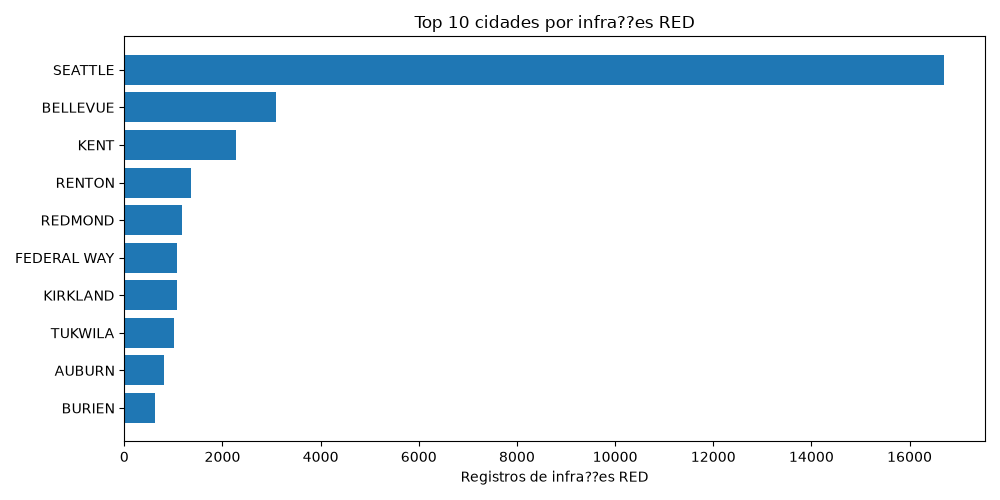
\includegraphics[width=0.85\linewidth]{grafico_q3.png}
  \caption{Top 10 cidades por registros de infrações RED.}
\end{figure}

\paragraph{Comentário.} A distribuição é fortemente concentrada: Seattle sozinha responde por quase metade (48,8\%) dos registros RED do condado, cerca de 5,4 vezes a segunda colocada (Bellevue). As 10 cidades somam 85,3\% do total, e a partir da quarta posição os valores caem para uma faixa estreita (1--4\%), formando uma cauda longa. O padrão acompanha o tamanho da cidade e a quantidade de estabelecimentos de alimentação, e não indica necessariamente que Seattle tenha restaurantes piores; para comparar a qualidade entre cidades seria necessário normalizar pelo número de inspeções ou de estabelecimentos.

% ---------------------------------------------------------------
\section{Evolução temporal}

Como cada linha é uma infração, contar linhas superestima o número de inspeções. Por isso foram calculadas, por ano, as inspeções únicas (\col{COUNT(DISTINCT inspection\_serial\_num)}), os registros de infração, os registros RED e as inspeções com ao menos uma infração RED.

\begin{lstlisting}[language=SQL]
SELECT year(inspection_date) AS year,
       COUNT(DISTINCT inspection_serial_num) AS unique_inspections,
       COUNT(violation_type) AS violation_records,
       SUM(CASE WHEN violation_type = 'RED' THEN 1 ELSE 0 END) AS red_records,
       COUNT(DISTINCT CASE WHEN violation_type = 'RED'
                           THEN inspection_serial_num END) AS inspections_with_red
FROM restaurant_violations
GROUP BY year(inspection_date)
ORDER BY year
\end{lstlisting}

\begin{table}[H]
\centering
\small
\caption{Inspeções e infrações por ano (2026 parcial, até 21/10).}
\begin{tabular}{lrrrrrr}
\toprule
Ano & Inspeções únicas & Reg. infração & Reg. RED & Insp. c/ RED & RED/inspeção & \% insp. c/ RED \\
\midrule
2021 & 6.433 & 4.280 & 2.230 & 1.565 & 0,35 & 24,3 \\
2022 & 9.837 & 8.906 & 4.562 & 3.024 & 0,46 & 30,7 \\
2023 & 12.302 & 13.106 & 6.692 & 4.217 & 0,54 & 34,3 \\
2024 & 14.785 & 15.314 & 7.461 & 4.710 & 0,50 & 31,9 \\
2025 & 16.418 & 15.581 & 7.813 & 5.059 & 0,48 & 30,8 \\
2026 & 14.354 & 11.870 & 5.486 & 3.469 & 0,38 & 24,2 \\
\bottomrule
\end{tabular}
\end{table}

\begin{figure}[H]
  \centering
  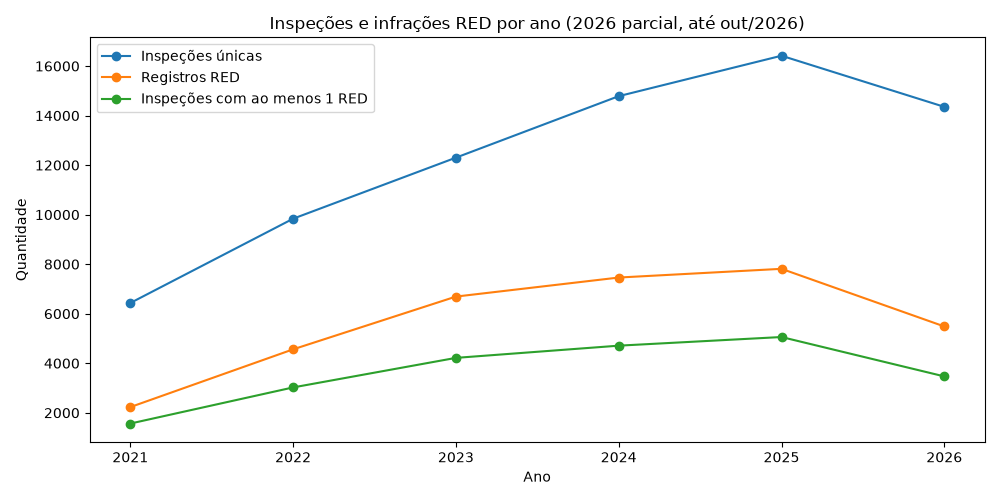
\includegraphics[width=0.85\linewidth]{grafico_q4.png}
  \caption{Inspeções únicas, registros RED e inspeções com ao menos uma infração RED por ano.}
\end{figure}

\paragraph{Discussão.}
\begin{itemize}
  \item \textbf{Volume de inspeções.} As inspeções únicas crescem continuamente de 6.433 (2021) para 16.418 (2025), cerca de 2,5 vezes. O valor baixo de 2021 é coerente com a retomada gradual das inspeções de rotina após as restrições da pandemia de COVID-19. Em 2026, com dados apenas até 21 de outubro, já são 14.354 inspeções, o que projeta um ano completo em torno de 17--18 mil; a queda no gráfico é efeito do ano incompleto, não uma redução real.
  \item \textbf{Infrações RED.} Os registros RED também crescem até 2025, mas em ritmo menor que as inspeções a partir de 2023. A taxa de registros RED por inspeção atinge o pico em 2023 (0,54) e cai para 0,48 em 2025 e 0,38 em 2026; a proporção de inspeções com ao menos uma RED segue o mesmo desenho (34,3\% em 2023 para 30,8\% em 2025 e 24,2\% em 2026). O aumento absoluto de RED reflete, portanto, principalmente o aumento de inspeções, enquanto a incidência relativa vem diminuindo desde 2023.
  \item \textbf{Registros versus inspeções únicas.} Em todos os anos há mais registros RED do que inspeções com RED: quando uma inspeção encontra uma infração RED, encontra em média 1,4 a 1,6 infrações RED. Em 2021, 2022 e 2025 o número de inspeções únicas é maior que o de registros de infração, já que muitas inspeções não registram nenhuma infração. Contar linhas, como no laboratório, mediria registros de infração e não inspeções.
\end{itemize}

% ---------------------------------------------------------------
\section{Execução distribuída}

Foi examinada na Spark UI a consulta da questão 4 executada pelo \col{by\_year.toPandas()} para gerar o gráfico (\textit{Query 15} na aba SQL/DataFrame). A sessão Livy completa gerou 42 jobs e 82 tasks (Figura~\ref{fig:jobs}).

\begin{figure}[H]
  \centering
  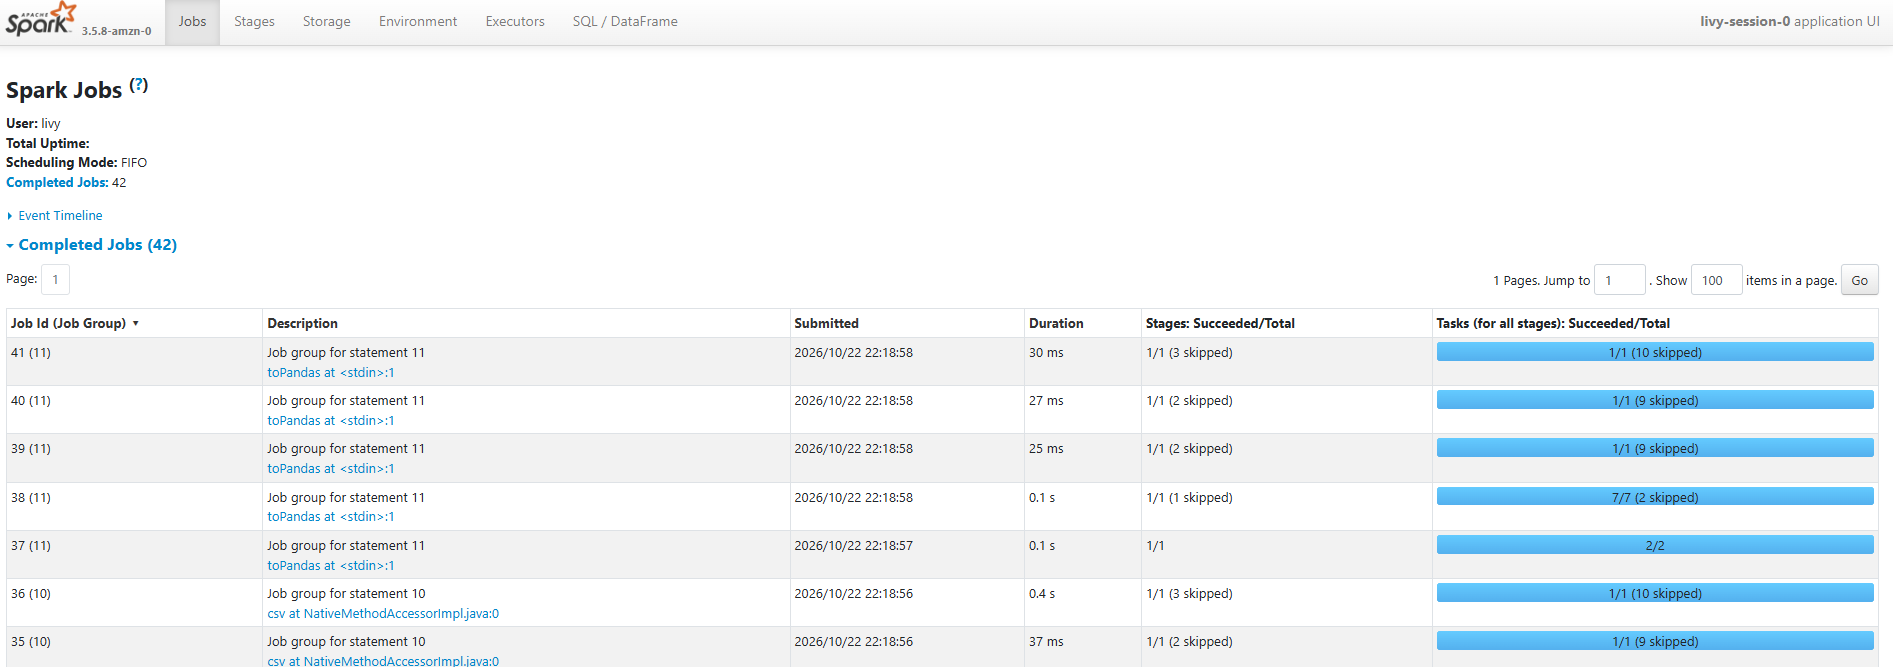
\includegraphics[width=\linewidth]{Jobs.png}
  \caption{Aba Jobs: jobs da sessão; os jobs 37 a 41 pertencem à consulta da questão 4.}
  \label{fig:jobs}
\end{figure}

\paragraph{Jobs.} A consulta gerou 5 jobs (37 a 41). Com a execução adaptativa (AQE), cada etapa de shuffle é materializada como um \textit{query stage} independente, disparado como um job; os jobs seguintes reaproveitam as etapas já concluídas, que aparecem como \textit{skipped}.

\paragraph{Stages.} Um stage é delimitado por cada operador \col{Exchange} (shuffle). O job 37 tem um único stage (70), que lê o DataFrame em cache, faz a agregação parcial e grava o shuffle (Figuras~\ref{fig:stage} e \ref{fig:dag}). O job 38 executa o stage seguinte, que lê esse shuffle (7 tasks) e conclui a agregação.

\begin{figure}[H]
  \centering
  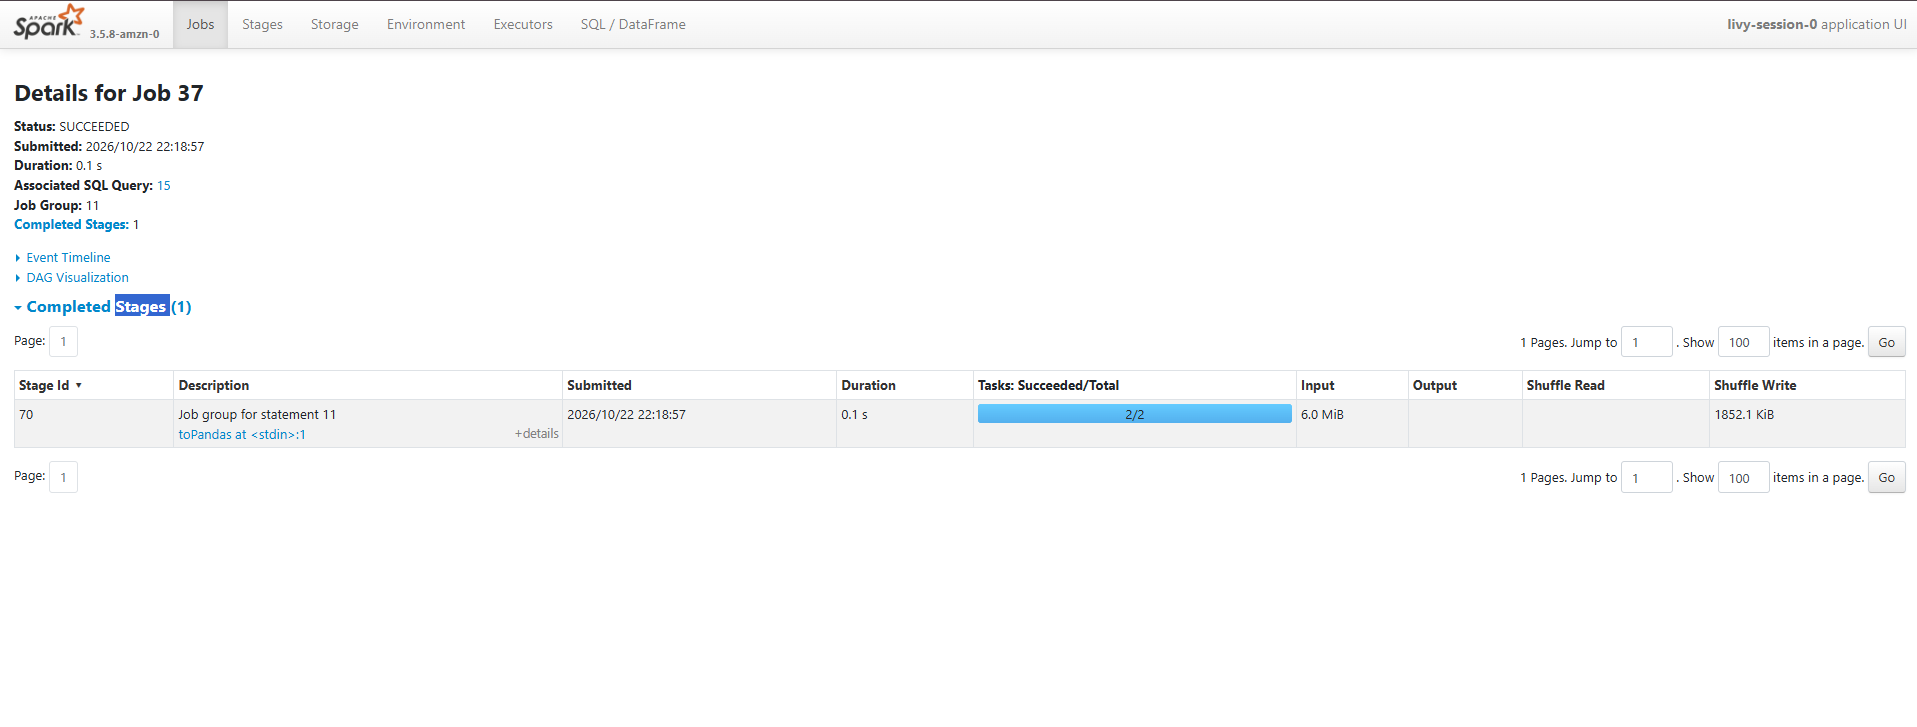
\includegraphics[width=\linewidth]{Stages.png}
  \caption{Job 37: um stage (70), 2 tasks, entrada de 6,0~MiB e 1.852,1~KiB de shuffle write.}
  \label{fig:stage}
\end{figure}

\begin{figure}[H]
  \centering
  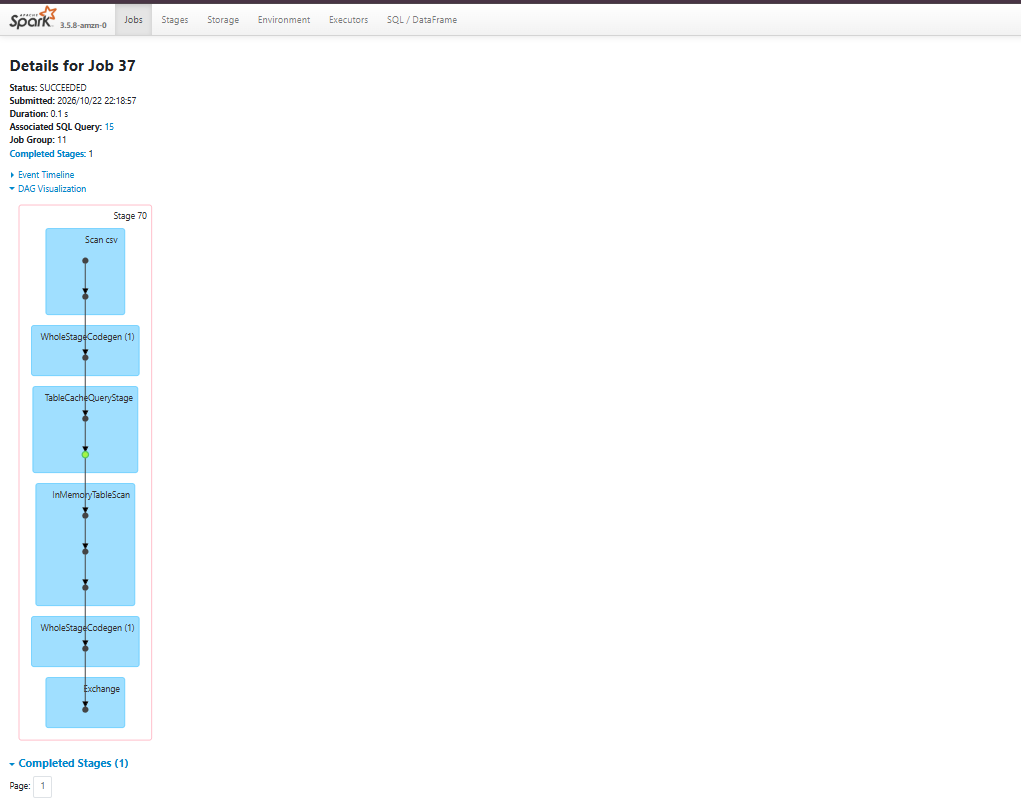
\includegraphics[width=0.55\linewidth]{dag_visualization.png}
  \caption{DAG do job 37: leitura do CSV/cache, \textit{whole-stage codegen} e \col{Exchange} ao final do stage 70.}
  \label{fig:dag}
\end{figure}

\paragraph{Tasks.} Cada partição gera uma task. O DataFrame tem 2 partições: o arquivo de 31,9~MB foi dividido pelo paralelismo padrão do cluster (\col{defaultParallelism} = 2, os 2 núcleos disponíveis). O stage 70 executou 2 tasks (71~ms e 89~ms), ambas no executor 1 (\col{ip-172-31-47-115}), com localidade \col{PROCESS\_LOCAL}, pois os dados já estavam em memória nesse executor. A entrada (``6,0~MiB / 12 records'') é contada em lotes colunares do cache, não em linhas. Juntas, as tasks gravaram 96.197 registros de shuffle (54.438 + 41.759), que são os resultados parciais da agregação.

\begin{figure}[H]
  \centering
  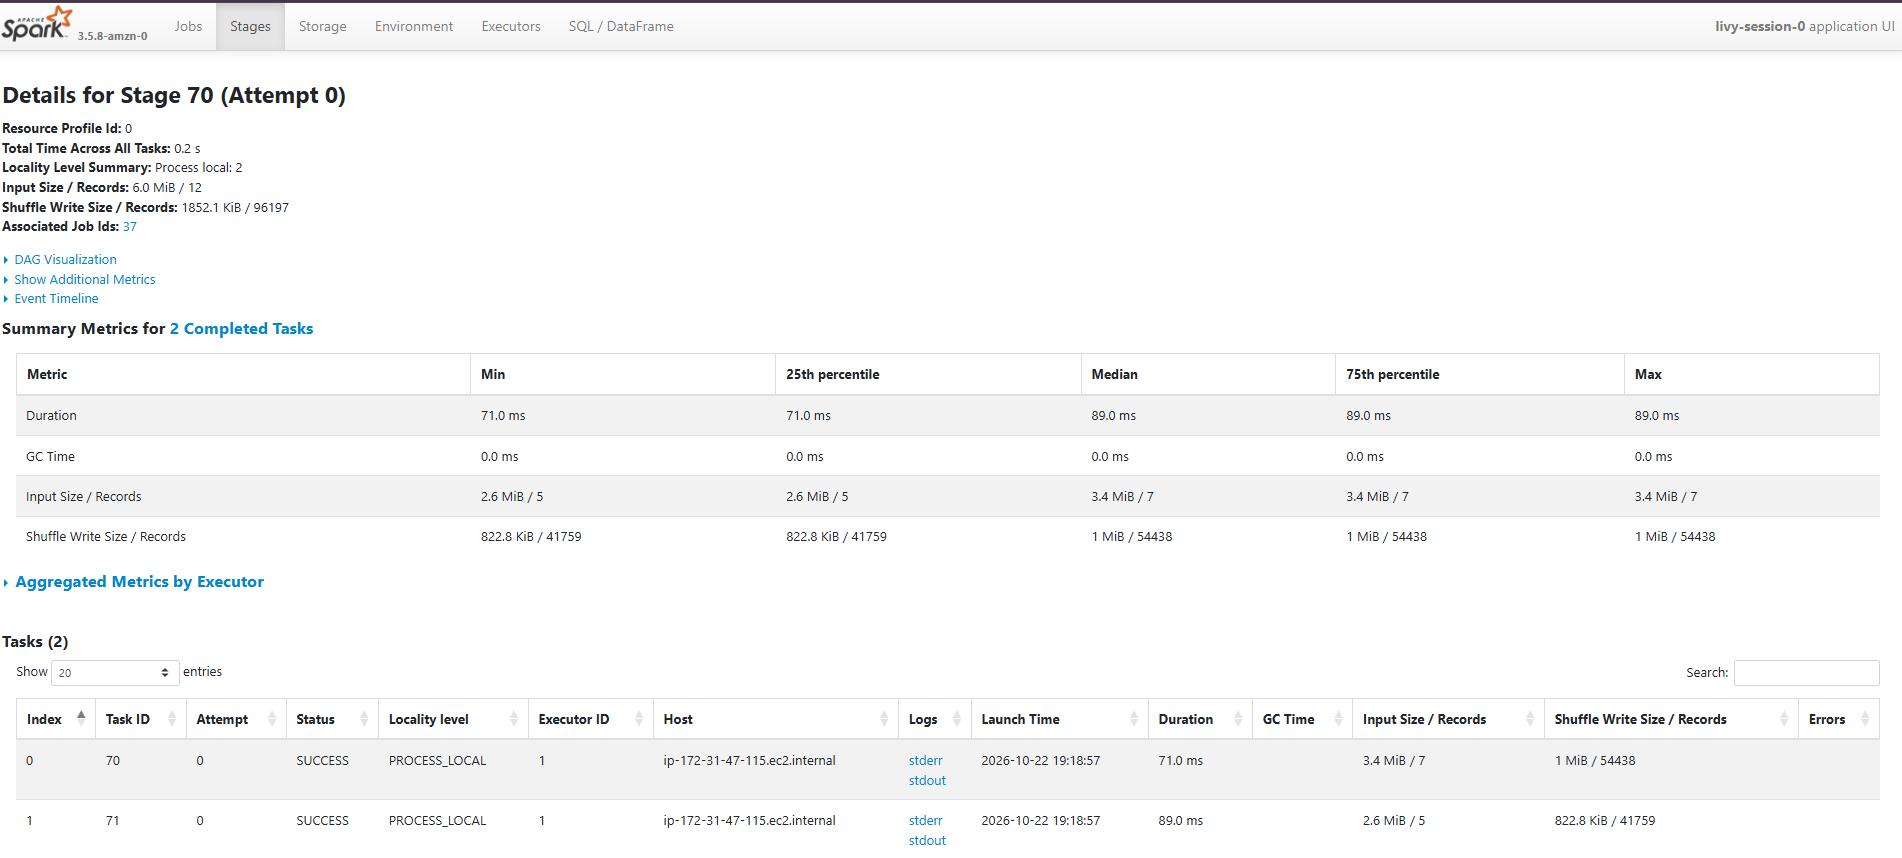
\includegraphics[width=\linewidth]{Tasks.png}
  \caption{Detalhes do stage 70: métricas resumidas e as 2 tasks.}
\end{figure}

\paragraph{Shuffle.} O plano físico (Figuras~\ref{fig:sql1}--\ref{fig:sql3}) mostra:
\begin{itemize}
  \item \col{InMemoryTableScan} lê as 110.068 linhas do cache.
  \item \col{Expand} triplica as linhas (330.204), pois a consulta tem duas agregações \col{COUNT(DISTINCT ...)}: cada linha é replicada uma vez por agregação distinta e uma vez para as agregações comuns.
  \item \col{HashAggregate} parcial reduz para 96.197 linhas em cada partição, antes da troca de dados.
  \item \textbf{Primeiro \col{Exchange}}: grava 96.197 registros (1.852,1~KiB) particionados pela chave de agrupamento. O plano inicial previa 1.000 partições de shuffle, mas o \col{AQEShuffleRead} as agrupou em apenas 7 (7,5~MiB), por serem pequenas, o que explica as 7 tasks do job 38. Toda a leitura foi local (\textit{local bytes read} = 1.852,1~KiB, \textit{fetch wait} = 0~ms).
  \item \col{HashAggregate} final e \textbf{segundo \col{Exchange}}: apenas 42 registros (6 anos $\times$ 7 partições) são redistribuídos para a agregação final por ano.
\end{itemize}

\begin{figure}[H]
  \centering
  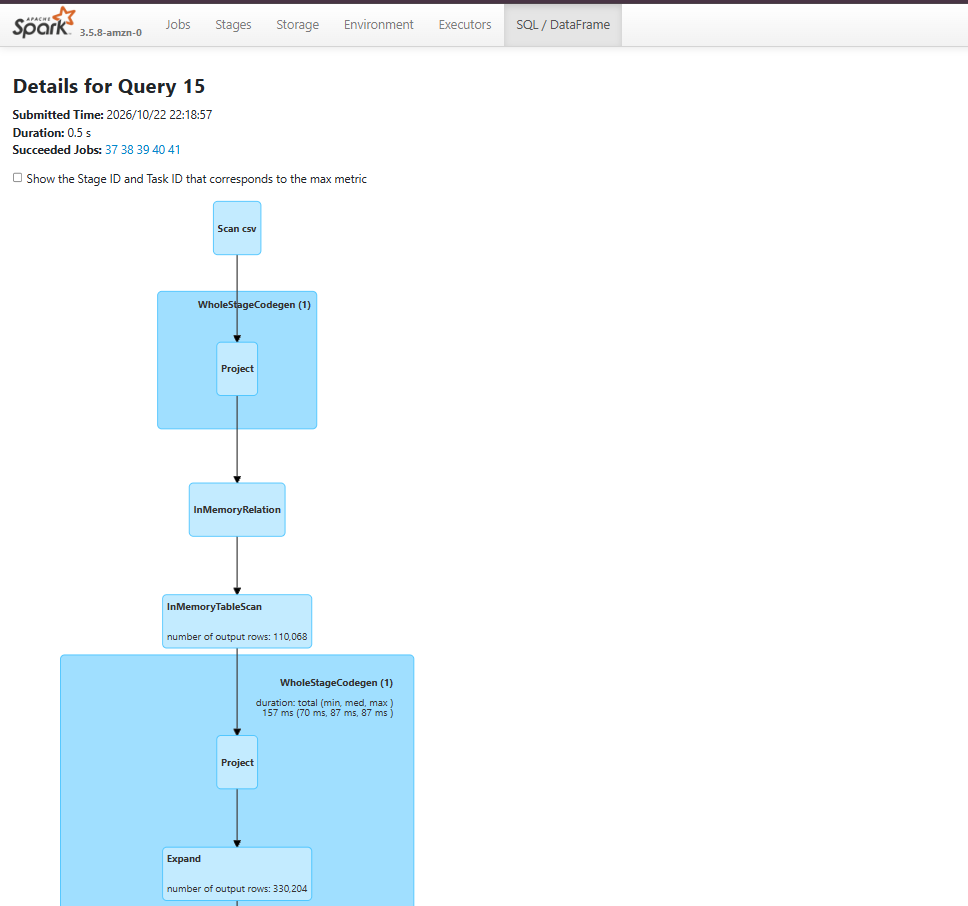
\includegraphics[width=0.6\linewidth]{SQL part1.png}
  \caption{Query 15 (parte 1): leitura do CSV, cache e \col{Expand}.}
  \label{fig:sql1}
\end{figure}

\begin{figure}[H]
  \centering
  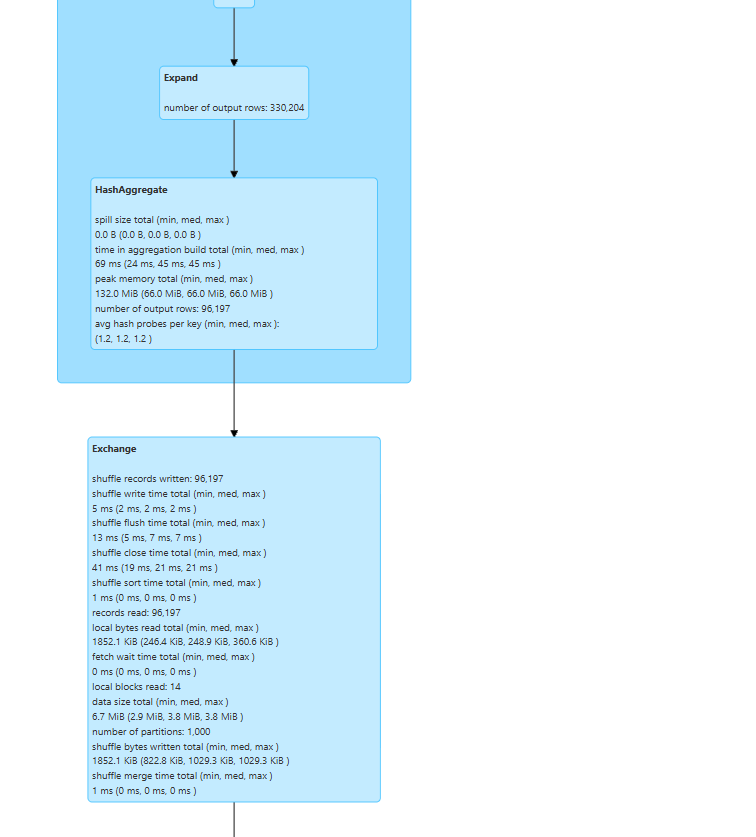
\includegraphics[width=0.6\linewidth]{SQL part2.png}
  \caption{Query 15 (parte 2): agregação parcial e primeiro \col{Exchange} (shuffle write/read).}
  \label{fig:sql2}
\end{figure}

\begin{figure}[H]
  \centering
  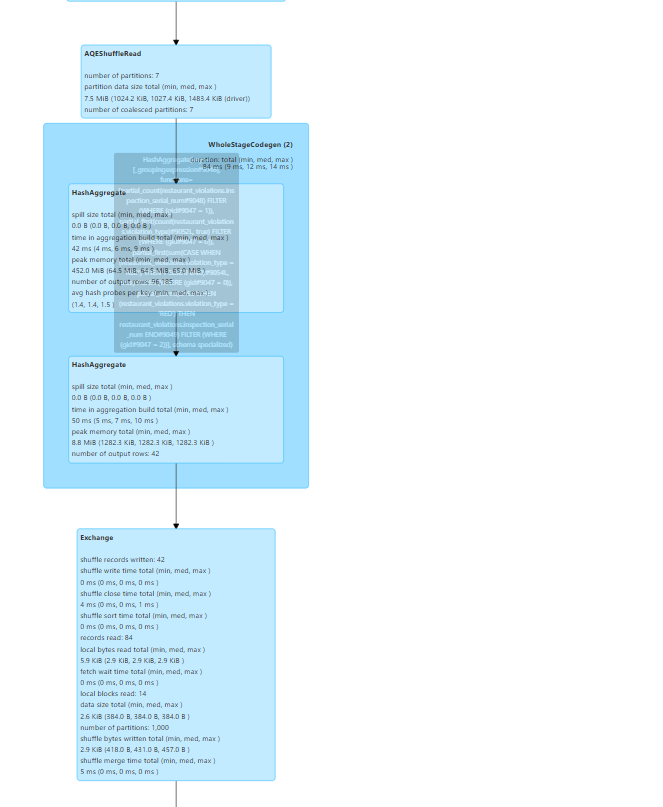
\includegraphics[width=0.6\linewidth]{SQL part3.png}
  \caption{Query 15 (parte 3): \col{AQEShuffleRead} com 7 partições, agregação final e segundo \col{Exchange}.}
  \label{fig:sql3}
\end{figure}

\paragraph{Executors.} A aba Executors (Figura~\ref{fig:exec}) mostra o \textit{driver} no nó primário (\col{ip-172-31-41-100}), responsável por planejar a consulta e agendar as tasks, sem executar nenhuma, e um único executor (ID~1) em um nó \textit{core} (\col{ip-172-31-47-115}), com 2 núcleos, que executou as 82 tasks da sessão (114,3~MiB lidos, 12,6~MiB de shuffle).

\begin{figure}[H]
  \centering
  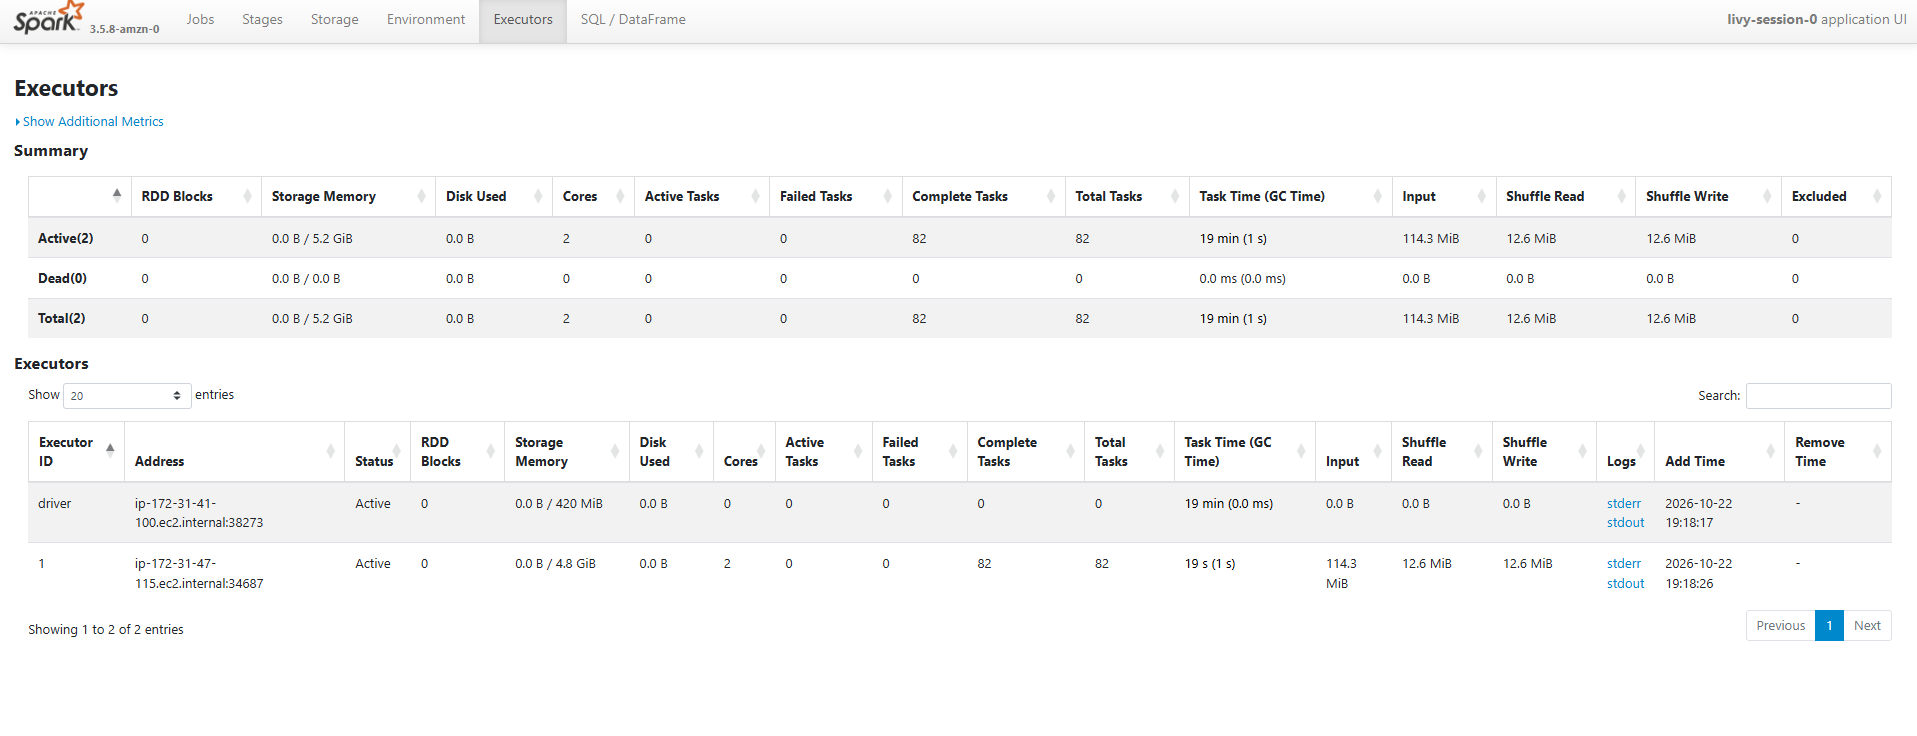
\includegraphics[width=\linewidth]{Executor_Tab.png}
  \caption{Aba Executors: driver e executor 1.}
  \label{fig:exec}
\end{figure}

\begin{figure}[H]
  \centering
  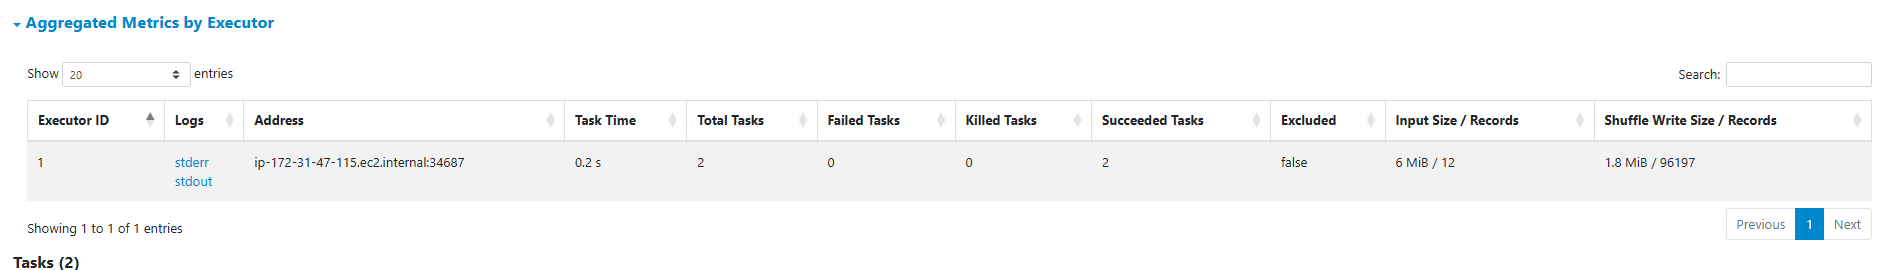
\includegraphics[width=\linewidth]{Executor.png}
  \caption{Métricas do stage 70 agregadas por executor.}
\end{figure}

\paragraph{Como o processamento foi distribuído.} O driver converteu a consulta SQL em um plano físico, dividiu-o em stages nos pontos de shuffle (\col{Exchange}) e enviou ao YARN uma task por partição. As tasks de cada stage rodaram em paralelo nos 2 núcleos do executor, e o shuffle redistribuiu os resultados parciais pela chave de agrupamento entre um stage e outro. Embora o cluster tenha 2 nós \textit{core}, apenas um executor foi alocado: o volume de dados é pequeno (2 partições de entrada) e as tasks duram dezenas de milissegundos, de modo que a alocação dinâmica do EMR não chegou a solicitar um segundo executor. Por isso o paralelismo efetivo foi de 2 tasks simultâneas e todo o shuffle foi local. Com um conjunto de dados maior, haveria mais partições, mais tasks pendentes e mais executores alocados, espalhando o processamento pelos dois nós e tornando o shuffle efetivamente transmitido pela rede.

\end{document}
